\documentclass{article}
\usepackage[utf8]{inputenc}


\usepackage{enumerate}
\usepackage{amsmath} % Tillater avansert formatering av matte.
\usepackage{amsfonts} % Tillater avanserte teikn, som R for reelle tall.
\usepackage{graphicx} % Tillater mer avansert formatering av grafikk.
\usepackage{geometry} % Tillater enklere formatering av sidevisning.
\usepackage{physics}
\usepackage{amssymb}
\setlength\parindent{0pt}

\title{Project 1}
\author{Johanne Mehren, Stine Sagen and Marit Kollstuen}


\begin{document}


\begin{abstract}
We present our Ferrari algorithm for solving linear equations. Our best algorithm runs as $4n$ FLOPS with $n$ the dimensionality of the matrix. \\
Use of linear algebra to solve linear equations and compare different methods and their 
\end{abstract}


\maketitle

\section{Introduction}
The main goal of project 1 is to develop a general algorithm for solving linear equations and implement a spesific matrix to our code. By testing two different ways to solve linear equations, we get a better understanding of how computers handle FLOPS, the relative error and running time. Compairing the exact solution to an approximation, we can see how step size is essential when you solve discretized problems. \\
The report gives a description of the theory behind the algorithm, a discussion about the results and a conclusion. \\ 
In our project we have used Python language, which does not require dynamic memory allocation. 


\section{Theory, algorithms and methods}
\subsection{Exact solution}
The one-dimensional Poisson equation is given by:
\begin{equation}\label{eq1} 
-u''(x) = f(x) 
\end{equation} 
To this equation, an exact (analytical) solutution does exist: 
\begin{equation}\label{eq2}
u(x) = 1 - (1-e^{-10})x - e^{-10x}
\end{equation}
when assuming the source term on the right hand side of \eqref{eq1} is defined as:
\begin{equation}\label{eq3}
f(x) = 100e^{-10x}
\end{equation} Substituting \eqref{eq2} into our differential equation \eqref{eq1}, we can then verify that this turns out to be correct:

\begin{align*}
u(x)& = 1 - (1-e^{-10})x - e^{-10x}  \\
u'(x)& = -1 + e^{-10} + 10e^{-10x} \\
u''(x)& = -100e^{-10x}  \\
-(-100e^{-10x})& = 100e^{-10x} \\
\therefore \\
100e^{-10x}& = 100e^{-10x}
\end{align*}

As expected, equation \eqref{eq2} is an exact solution of the Poisson equation \eqref{eq1}. 

\medskip

Our differential equation concernes a boundary value problem which means our solution also needs to satisfy the given boundary conditions given by:
\begin{equation}\label{eq4}
u(0) = u(1) = 0
\end{equation}

Checking the behavior of the exact solution at its boundary points:

\begin{align*}
u(0)& = 1-(1-e^{-10})\cdot 0 -e^{-10\cdot 0} = 0 \\
u(1)& = 1-(1-e^{-10})\cdot 1 -e^{-10\cdot 1} = 0 \\
\end{align*}

Equation \eqref{eq2} is a solution of our boundary value problem.

\medskip

As mentioned in the introduction, we want to compare this exact solution with the numerical solution we obtain when the boundary value problem takes a discretized form. 

\subsection{Finite difference method}

We want to solve the Poisson equation \eqref{eq1} numerically. This can be achived by using something we call finite-difference methods. When using finite-difference methods, we are replacing the derivatives appearing in the differential equation by finite difference approximations at a given set of discrete points in space and/or time. When this method is applied to the second order derivative in the Poisson equation \eqref{eq1}, we obtain a dicretized approximation for u in the x-direction because its only depended on the spacial variable x.  

\medskip

A way to find these finite difference approximations is by using Taylor series expansion on the function $u(x)$. 

\subsubsection{Taylor series expansion}

The derivative of a function u(x) is defined as:

\begin{equation}
\frac{dfu(x)}{dx} = \lim_{h \to 0} \frac{u(x+h) - u(x)}{h}
\end{equation}

where h is the step length. Further a Taylor expansion forward and backward in the spacial direction x can be done: 

\begin{align*}
u(x+h)& = u(x) + hu' + \frac{h^2u''}{2!}  + \frac{h^3u'''}{3!} + O(h^4)\\
u(x-h)& = u(x) - hu' +  \frac{h^2u''}{2!} -\frac{h^3u'''}{3!} + O(h^4)
\end{align*}

where the first equation is expanded forward and the second backward in space.  

\medskip

To obtain finite difference approximation for the second order derivative we then sum the two equations:

\begin{align*}
u(x+h) + u(x-h)& = 2u(x) + \frac{2h^2u''}{2!} + O(h^4) 
\end{align*}

where the h inside of the big O-notation is the truncation error.
Solving for $u''$ we then end up with the following equation:

\begin{equation}
u'' = \frac{u(x+h) + u(x-h) -2u(x)}{h^2} + O(h^2)
\end{equation}

We see that the truncation error is of second order $(h^2)$.  This error that arises when truncating the derivatives with Taylor series. Further, this result will now be applied to our spesific boundary value problem. 

\subsubsection{Discretization of the boundary value problem}

As mentioned above,  the concept of discretizing is about dividing the domain into a finite set of discrete points. We now the discretize $u$ as $v_i$ with grid points $x_i =  ih$  in the range from $x_0= 0$ to $x_{n+1}=1$. The grid spacing is defined as $h = \frac{x_{n+1}-x_0}{n+1} = \frac{1}{n+1}$.  Our approximated finite difference approximation for equation \eqref{eq1} is now:

\begin{equation}\label{eq7}
-\frac{v_{i+1} + v_{i-1} -2v_i}{h^2} = f_i
\end{equation}

with the boundary conditions: $v_0 = v_{n+1} = 0$ and $i = 1,...,n$.  

\medskip


By using algebraic methods, the equation \eqref{eq7} must first be rewritten into a set of linear equations. Assuming $n= 4$, it can be shown that this can be represented as a Toepliz-matrix by setting: 

\[
	v
=
\begin{bmatrix}
	 v_1 & v_2 & v_3 & v_4
\end{bmatrix}
\]

In which 

\[
\begin{bmatrix}
	v_1" \\  v_2" \\ v_3" \\ v_4"
\end{bmatrix}
	\approx -\frac{1}{h^2}
\begin{bmatrix}
	-(v_{0} -2v_1 +v_2) \\
	-(v_1 -2v_2 +v_3) \\
	-(v_{2} -2v_3 +v_4) \\
	-(v_{3} -2v_4 +v_5) 
\end{bmatrix}
\]

The boundary conditions are set to $v_0 = v_{n+1} = 0$, so the expression becomes: 

\[
\begin{bmatrix}
	2 & -1 & 0 & 0 \\
	-1 & 2 & -1 & 0 \\
	0 & -1 & 2 & -1 \\
	0 & 0 & -1 & 2
\end{bmatrix}
\begin{bmatrix}
	v_1 \\  v_2 \\ v_3 \\ v_4
\end{bmatrix}
	= -h^2
\begin{bmatrix}
	f_1 \\
	f_2 \\
	f_3 \\
	f_4
\end{bmatrix}
\]

In which $f_i$ is known. 



\subsection{A general algorithm for solving the tridiagonal matrix}
To obtain a numerical solution to the second order derivative of $u(x)$, the method of gaussian ellimination is used to solve the set of linear equations given by: . 
Gaussian ellimination is based on two stages, namely forward substitution and a backward substitution. The first equation is used to eliminate the first uknown vector element $v1$ from the remaining n-1 equations. The second equation (which is changed) is used to eliminate $v2$ from the remaining n-2 equations and so on. This stage is the forward substitution. In the backward substitution stage, the equations are solved recursively starting from $v_n$ up to first uknown vector element $v_1$. \\ We are in our case dealing with a tridiagonal matrix where all the elements are zero except the diagonal and the elements just above and below this. Our function for the algorithm takes four parameters: a (below diagonal element), b (diagonal element), c (upper diagonal element) and n which is the amount grid points we want to test for. In addition, the solution vector \textbf{v} is stored in \textbf{v{\_}vec}, the source term as $\textbf{f\textunderscore{vec}} = h^2f(x)$ and \textbf{b} as \textbf{b{\_}vec}.
A piece of the generalized algorithm (assuming different values of a,b and c) is given here: 
\\\\
Forward substitution:\\
$i=0:n-2$
\begin{align*}
b\textunderscore{vec}[i+1] & \leftarrow b\textunderscore{vec}[i+1]  - \frac{a \cdot c}{b\textunderscore{vec}[i]}     (\sim update)\\
f\textunderscore{vec}[i+2] &\leftarrow f\textunderscore{vec}[i+2]  - \frac{a \cdot f\textunderscore{vec}[i+1]}{b\textunderscore{vec}[i]}      (\sim update)\\
\end{align*}
Backward substitution: \\
$i = n:1 $
\begin{align*}
f\textunderscore{vec}[i-1] & \leftarrow f\textunderscore{vec}[i-1] - \frac{c \cdot f\textunderscore{vec}[i]}{b\textunderscore{vec}[i-1]}      (\sim update)\\
\end{align*}
Solution vector:\\
$i =1:n$
\begin{align*}
v\textunderscore{vec}[i] & = \frac{f\textunderscore{vec}[i]}{b\textunderscore{vec}[i-1]}
\end{align*}

\subsection{Specialized algorithm for solving the tridiagonal matrix}
For the special case let $a = -1$, $b = 2$ and $c = -1$ be the values of the respective elements in the tridiagonalmatrix given in (). This function takes the parameters a,b and n. The specialized algorithm can be intepreted as follows: \\
Forward substitution:\\
$i=0:n-2$
\begin{align*}
b\textunderscore{vec}[i+1] & \leftarrow b\textunderscore{vec}[i+1]  - \frac{a^2}{b\textunderscore{vec}[i]}     (\sim update)\\
f\textunderscore{vec}[i+2] &\leftarrow f\textunderscore{vec}[i+2]  - \frac{a \cdot f\textunderscore{vec}[i+1]}{b\textunderscore{vec}[i]}      (\sim update)\\
\end{align*}
Backward substitution: \\
$i = n:1 $
\begin{align*}
f\textunderscore{vec}[i-1] & \leftarrow f\textunderscore{vec}[i-1] - \frac{a \cdot f\textunderscore{vec}[i]}{b\textunderscore{vec}[i-1]}      (\sim update)\\
\end{align*}
Solution vector:\\
$i =1:n$
\begin{align*}
v\textunderscore{vec}[i] & = \frac{f\textunderscore{vec}[i]}{b\textunderscore{vec}[i-1]}
\end{align*}

\subsection{Relative error}

By analyzing the relative error, we can approximate a minimal step length that does not lead to loss of precision due to subtraction of near-equal numbers. The relative error between the analytical and the numerical solution can be defined as:

\begin{equation}
	\epsilon_{i} = log_{10}\bigg(\abs{\frac{v_i-u_i}{u_i}}\bigg)
	\label{eq:8}
\end{equation}

as a function of $log_{10}(h)$.

\subsection{LU Decomposition}
The concept of gaussian ellimination gives rise to another often used method called LU decomposition method. Using this method, the matrix $\textbf{A}$ can be decomposed into the product of two matrices L and U, where L only has elements below the diagonal and U has elements  both at diagonal and the upper diagonal. On matrix form the decomposition of $\textbf{Av} = \textbf{f}$ can be intepreted like:
\begin{equation} 
\label{lu}
 \textbf{Av} = \textbf{LUv} = \textbf{f}
\end{equation}
Equation (\ref{lu}) is then computed in two steps:
\begin{equation}
\label{lu_dec}
\textbf{Ly} = \textbf{f},     \quad  \textbf{Uv} = \textbf{y} 
\end{equation}
where \textbf{y} is assumed to be another vector of same length as \textbf{v} which is used to calculate the second equation in  (\ref{lu_dec}) and thereby the wanted solution for \textbf{v}.

\section{Results}

% CPU time 
In  table \ref{tab:1}, the different CPU times for the developed algorithms in addition to the LU-decomposition are shown for different choices of grid points n. When n increaces, the computational time slows down. Clearly, the LU-decomposition is the slowest algorithm. When n is equal to $10^4$ ($n>10^4$ in LU method does not work) it uses approximately 14.26 seconds compared to the general and special one which use 0.03234 and 0.03215 seconds for performing the same calculations. There is not a huge difference between the general and special algorithm in the computation time, nevertheless, the general uses sligtly longer time compared to the other. 

\begin{table}[]
\begin{tabular}{llll}
           & \multicolumn{3}{c}{\textbf{Time (s):}}                                                                  \\ \hline
           & \textbf{Gaussian elimination (g.a.):} & \textbf{Gaussian elimination (s.a.):} & \textbf{LU-decomposition:} \\ \hline
n = $10$   & $4.816e-05$                              & $4.196e-05$                              & $0.0001301$       \\
n = $10^2$  & $0.0003078$                              & $0.0002770$                              & $0.0002670$       \\
n = $10^3$ & $0.003332$                               & $0.003214$                               & $0.02403$         \\
n = $10^4$ & $0.03234$                                & $0.03215$                                & $14.26$           \\
n = $10^5$ & $0.3629$                                 & $0.3458$                                 & N/A               \\
n = $10^6$ & $3.109$                                  & $3.136$                                  & N/A               \\
n = $10^7$ & $32.79$                                  & $32.20$                                  & N/A              
\end{tabular}
\label{tab:1}
\caption{CPU-time for the different algorithms (g.a. = general algorithm, s.a. = special algorithm)}
\end{table}


\begin{figure}[h]
    \centering
    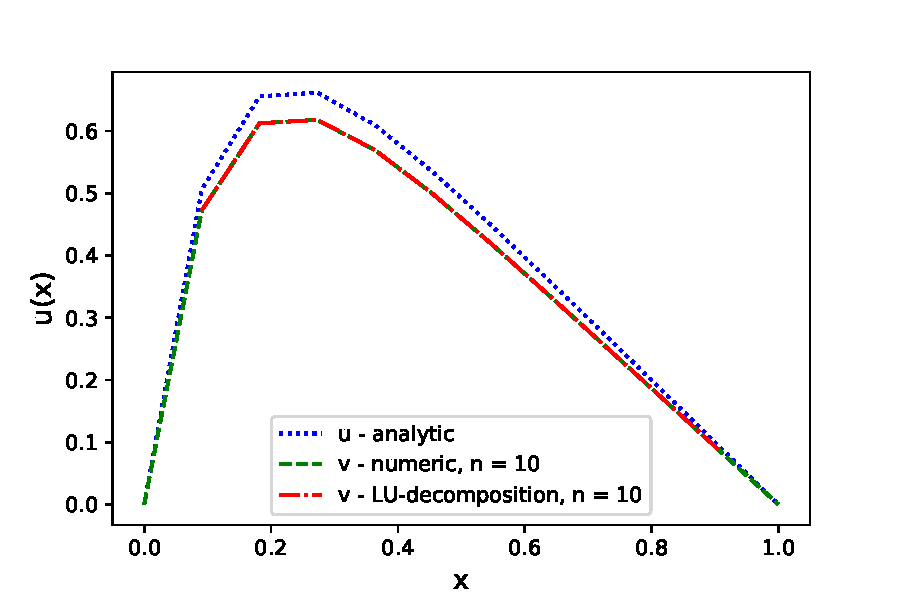
\includegraphics[width =12cm]{python/size_10.pdf}
    \caption{Size 10}
    \label{fig:1}
\end{figure}

\begin{figure}[h]
    \centering
    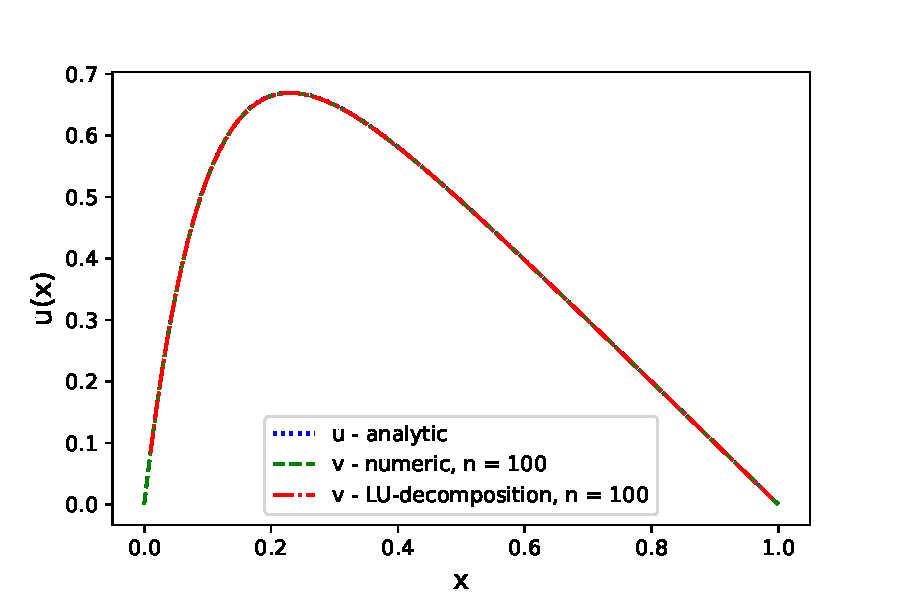
\includegraphics[width =12cm]{python/size_100.pdf}
    \caption{Size 100}
    \label{fig:2}
\end{figure}


\begin{figure}[h]
    \centering
    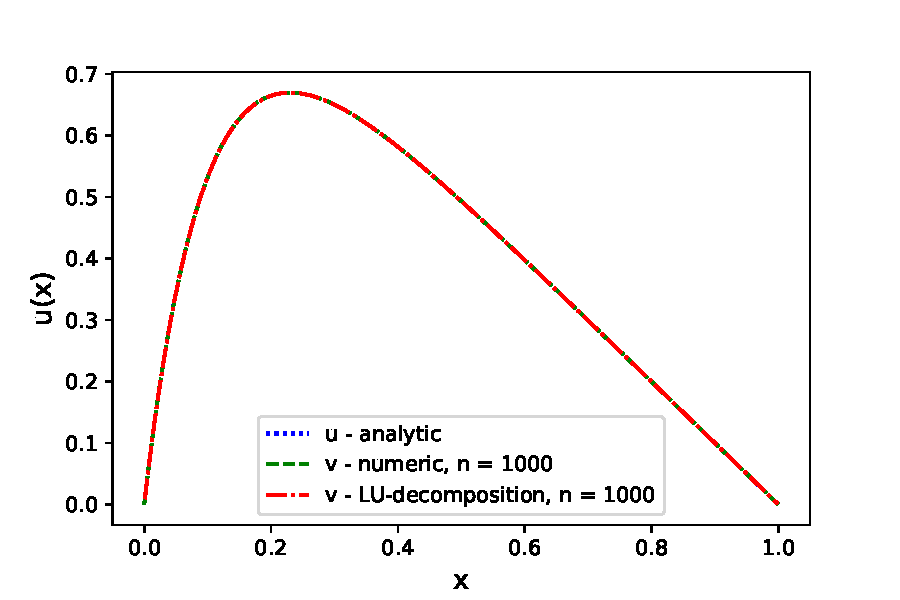
\includegraphics[width =12cm]{python/size_1000.pdf}
    \caption{Size 1000}
    \label{fig:3}
\end{figure}


\begin{figure}[h]
    \centering
    \includegraphics[width =12cm]{python/size_10000.pdf}
    \caption{Size 10000}
    \label{fig:4}
\end{figure}

Table \ref{tab:2} contains the maximal (in absolute value) relative error defined by Equation \ref{eq:8}. This shows that the relative error is decreasing for decreasing $h$ (increasing $n$) until $h = 10^{-5}$, at which the relative error is at it's lowest and after which it increases again. The relative error is displayed as a function of the stepsize, $h$, in Figure \ref{fig:re}. This confirms that a smaller stepsize to a certain degree relates to a smaller relative error. Thus a loss of precision can be avoided by making the stepsize smaller. 

\begin{table}[]
\centering
\begin{tabular}{ll}
\multicolumn{2}{c}{\textbf{Max. relative error, $\epsilon_{max}$:}} \\ \hline
n = $10$                                  & $-1.1797$                                \\
n = $10^2$                                & $-3.08804$                               \\
n = $10^3$                                & $-5.08005$                               \\
n = $10^4$                                & $-7.07928$                               \\
n = $10^5$                                & $-8.84298$                                \\
n = $10^6$                                & $-6.07550$                               \\
n = $10^7$                                & $-5.52523$                              
\end{tabular}
\label{tab:2}
\caption{Relative error for the specialized algorithm using Equation \ref{eq:8}}
\end{table}


\begin{figure}[h]
    \centering
    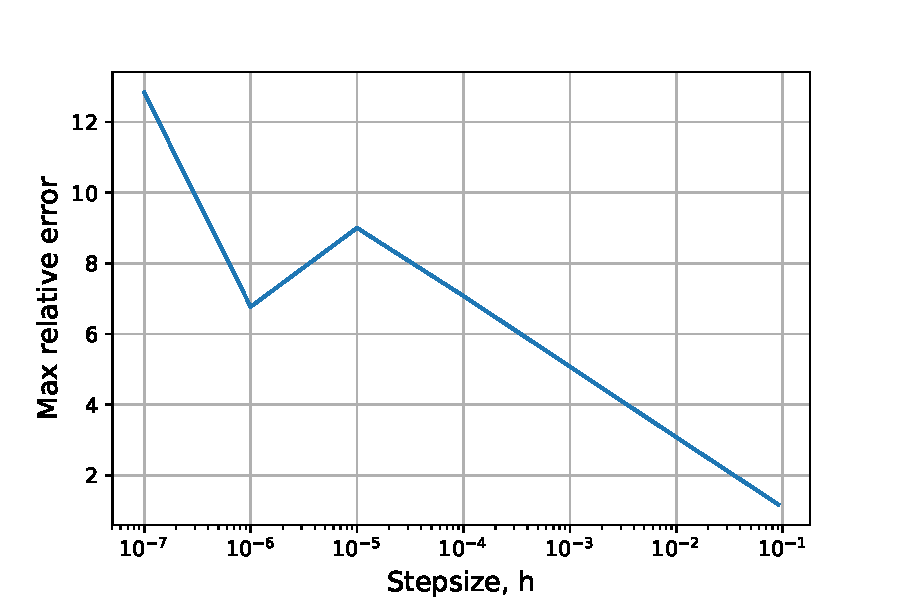
\includegraphics[width =12cm]{python/relative_error.pdf}
    \caption{Log-log plot or the relative error of the second derivative of $u(x)$ (Equation \ref{eq2}}
    \label{fig:re}
\end{figure}


\section{Conclusion}

\section{References}


\end{document}